% !TEX TS-program = pdflatex
% !TeX program = pdflatex
% !TEX encoding = UTF-8
% !TEX spellcheck = fr

\documentclass[xcolor=table]{beamer}

\input{options}

\title[TALN : 03- ML pour TALN]%
{Traitement automatique du langage naturel\\Chapitre 03 : Apprentissage automatique pour TALN} 

\changegraphpath{../img/ml4nlp/}

\begin{document}
	
%	\begin{frame}
%		\frametitle{Traitement automatique du langage naturel}
%		\framesubtitle{ML pour TALN : Introduction}
%		
%		
%	\end{frame}
	
	\begin{frame}
		\frametitle{Traitement automatique du langage naturel}
		\framesubtitle{ML pour TALN : Algorithmes}
		
		\begin{itemize}
			\item \optword{NB} (Naive Bayes)
			\item \optword{LR} (Logistic regression) : Régression logique
			\item \optword{SVM} (Support-Vector Machine) : Machines à vecteurs de support 
			\item \optword{NN} (Neural Network) : Réseau de neurones
			\item \optword{FFN} (Feed Forward Network) : Réseau à propagation avant
			\begin{itemize}
				\item \optword{MLP} (Multi-Layer Perceptron) : Perceptron multicouche
				\item \optword{CNN} (Convolutional Neural Network) : Réseau de neurones convolutif
			\end{itemize}
			\item \optword{RNN} (Recurrent Neural Network) : Réseau de neurones récurrents
			\item \optword{HMM} (Hidden Markov Model) : Modèle de Markov caché
			\item \optword{MEMM} (Maximum-Entropy Markov Model) : Modèle de Markov à entropie maximale
			\item \optword{CRF} (Conditional Random Field) : Champ aléatoire conditionnel
		\end{itemize}
		
	\end{frame}
	
	\begin{frame}
		\frametitle{Traitement automatique du langage naturel}
		\framesubtitle{ML pour TALN : Types des modèles}
		
		\scriptsize
		\begin{tblr}{
				colspec = {p{.12\textwidth}lp{.37\textwidth}lp{.38\textwidth}},
				row{odd} = {lightblue},
				row{1} = {darkblue, fg=white, font=\bfseries, valign=m, halign=c},
				column{2,4}={white},
				column{1}={bg=darkblue, fg=white, font=\bfseries, valign=m},
				row{even} = {white},
				cell{1}{1}={white},
				colsep=3pt,
				rowsep=1pt,
			}
			
			&& Génératif && Discriminatif \\
			
			&&&&\\
			
			Texte && NB && LR, SVM, MLP, RNN, CNN \\
			
			&&&&\\
			
			Séquence && HMM  && MEMM, CRF, RNN \\
			
		\end{tblr}
		
		\vfill
		
		\begin{itemize}
			\item Modèle génératif : un modèle qui apprend à générer des caractéristiques étant donnée la classe
			
			$\hat{Y} = \arg\max_k P(Y_k) P(X | Y_k)$
			
			\item Modèle discriminatif : un modèle qui apprend à estimer la classe directement 
			
			$\hat{Y} = \arg\max_k P(Y_k | X)$
			
			
		\end{itemize}
		
	\end{frame}
	
	
	\begin{frame}
		\frametitle{Traitement automatique du langage naturel}
		\framesubtitle{ML pour TALN : Plan}
		
		\begin{multicols}{2}
			%	\small
			\tableofcontents
		\end{multicols}
	\end{frame}
	
	%===================================================================================
	\section{Apprentissage automatique}
	%===================================================================================
	
	\begin{frame}
		\frametitle{ML pour TALN}
		\framesubtitle{\insertsection}
		
	\end{frame}
	
	\subsection{ML traditionnel}
	
	\begin{frame}
		\frametitle{ML pour TALN : \insertsection}
		\framesubtitle{\insertsubsection\ : Naive Bayes}
		
		Classement 
		\[\hat{Y} = \arg\max_{Y_k} \log P(Y_k) + \sum_{j=1}^{N} \log P(X_j|Y_k)\]
		
		Apprentissage
		\[P(Y_k) = \frac{|\{y / y \in Y \wedge y = k\}|}{M}\]
		
		\begin{itemize}
			\item $|\{y / y \in Y \wedge y = k\}|$ est le nombre des échantillons appartenant à la classe $k$ dans le dataset d'entraînement
			\item $M$ est le nombre des échantillons dans le dataset d'entraînement
			\item $P(X_j|Y_k)$ est calculée selon une des trois lois : lois multinomiale, lois normale et lois de Bernoulli
		\end{itemize}
		
	\end{frame}
	
	\begin{frame}
		\frametitle{ML pour TALN : \insertsection}
		\framesubtitle{\insertsubsection\ : Régression logistique}
		
		Classement 
		\[\hat{Y} = \arg\max_{k} Softmax(\sum_{j=1}^{N} \theta_j X_j + \theta_0)\]
		
		Apprentissage
		\[J_\theta = \frac{-1}{M} \sum\limits_{i=1}^{M} \sum_{k=1}^{L} Y^{(i)}_k \log(H^{(i)}_k)\]
		\[\theta_j = \theta_j - \alpha \frac{\partial J_\theta}{\partial \theta_j}\]
		
		\begin{itemize}
			\item $\theta$ est mis à jours avec un algorithme d'optimisation comme la \keyword{descente du gradient}
			\item $\theta[N, K]$ est une matrice de $N$ caractéristiques et $K$ classes
		\end{itemize}
		
	\end{frame}
	
	\begin{frame}
		\frametitle{ML pour TALN : \insertsection}
		\framesubtitle{\insertsubsection\ : Machine à vecteur de support}
		
		Classement 
		\[\hat{Y_t} = \arg\max_{k} \sum^M_{i=1} \alpha^k_i y^{(i)} K(x^{(i)}, x_t) - b^k\]
		
		Apprentissage
		\[J_\alpha = \sum\limits_{i=1}^{M} \alpha_i - \frac{1}{2} \sum\limits_{i=1}^{M} \sum\limits_{j=1}^{M} \alpha_i \alpha_j y^{(i)} y^{(j)} K(x^{(i)}, x^{(j)}) \]
		
		\begin{itemize}
			\item $\alpha$ est mis à jours avec un algorithme d'optimisation comme la \keyword{Sequential minimal optimization}
		\end{itemize}
		
	\end{frame}
	
	\subsection{MLP}
	
	\begin{frame}
		\frametitle{ML pour TALN : \insertsection}
		\framesubtitle{\insertsubsection}
		
		\vgraphpage{RN.pdf}
		
	\end{frame}
	
	\begin{frame}
		\frametitle{ML pour TALN : \insertsection}
		\framesubtitle{\insertsubsection\ : Architecture}
		
		\vgraphpage{RNPA.pdf}
		
	\end{frame}
	
	
	\subsection{CNN}
	
	\begin{frame}
		\frametitle{ML pour TALN : \insertsection}
		\framesubtitle{\insertsubsection : traitement d'image traditionnel}
		
		\begin{center}
			\hgraphpage[\textwidth]{img-learn.pdf}
		\end{center}
		
	\end{frame}
	
	\begin{frame}
		\frametitle{ML pour TALN : \insertsection}
		\framesubtitle{\insertsubsection\ : convolution (principe)}
		
		\begin{itemize}
			\item Une image est une matrice des pixels
			\item Convolution : modifier la valeur d'un pixel par rapport à ces voisins
			\item deux paramètres : \optword{padding} (entourer l'image avec des 0 afin de préserver la taille originale), \optword{stride} (le pas de défilement du noyau/masque)
		\end{itemize}
		
		\begin{center}
			\hgraphpage[.8\textwidth]{conv.pdf}
		\end{center}
		
	\end{frame}
	
	\begin{frame}
		\frametitle{ML pour TALN : \insertsection}
		\framesubtitle{\insertsubsection\ : Conv2D}
		
		\begin{minipage}{0.60\textwidth} 
			\begin{itemize}
				\item On préserve la structure spatiale des images
				\item La couche apprend un ou plusieurs noyaux
				\item $ w' = \frac{w - w_f + 2P}{S} + 1$,  $ h' = \frac{h - h_f + 2P}{S} + 1$
				\item On peut spécifier le nombres des filtres $k$ à générer 
				\item Le nombre des paramètres sera $w_f * h_f * c * k$ plus $k$ biais
				\item Exemple, \expword{image : 32x32x3; noyau : 5x5; s : 1; p: 0; k : 6.} Dans ce cas, on aura \expword{81} paramètres à entraîner
			\end{itemize}
		\end{minipage}
		%
		\begin{minipage}{0.39\textwidth}
			\hgraphpage[\textwidth]{conv2d.pdf}
		\end{minipage}
		
	\end{frame}
	
	\begin{frame}
		\frametitle{ML pour TALN : \insertsection}
		\framesubtitle{\insertsubsection\ : Pooling}
		
		\begin{minipage}{0.60\textwidth} 
			\begin{itemize}
				\item Rendre la représentation plus petite et plus gérable
				\item $ w' = \frac{w - w_f + 2P}{S} + 1$,  $ h' = \frac{h - h_f + 2P}{S} + 1$
				\item Pas de paramètres 
				\item \optword{Max Pool} : le gradient est passé seulement à la cellule gagnante (qui a le max) 
				\item \optword{Average Pool} : le gradient passé aux cellules participantes à la moyennes est $\frac{\text{gradient}}{w_f * h_f}$ 
			\end{itemize}
		\end{minipage}
		%
		\begin{minipage}{0.39\textwidth}
			\hgraphpage[\textwidth]{maxpool.pdf}
		\end{minipage}
		
	\end{frame}
	
	\subsection{RNN}
	
	\begin{frame}
		\frametitle{ML pour TALN : \insertsection}
		\framesubtitle{\insertsubsection\ : Architecture}
		
		\begin{minipage}{0.49\textwidth} 
			\begin{itemize}
				\item \optword{Elman network}
				\begin{align*}
					h_t = f(w_x x_t + w_h \textcolor{red}{h_{t-1}} + b_h) \\
					\hat{y}_t = g(w_y h_t + b_y)
				\end{align*}
				\item \optword{Jordan network}
				\begin{align*}
					h_t = f(w_x x_t + w_h \textcolor{red}{\hat{y}_{t-1}} + b_h) \\
					\hat{y}_t = g(w_y h_t + b_y)
				\end{align*}
			\end{itemize}
		\end{minipage}
		%
		\begin{minipage}{0.5\textwidth}
			\hgraphpage[\textwidth]{RNN.pdf}
		\end{minipage}
		
	\end{frame}
	
	\begin{frame}
		\frametitle{ML pour TALN : \insertsection}
		\framesubtitle{\insertsubsection\ : Applications}
		
		\begin{tabular}{p{.32\textwidth}p{.15\textwidth}p{.4\textwidth}}
			\hline\hline
			Type & Illustration & Exemple \\
			\hline
			Plusieurs à plusieurs & 
			\vgraphpage[1.5cm, valign=c]{RNNpp1.pdf} & 
			Détection d'entités nommées \\
			
			\hline
			Plusieurs à plusieurs & 
			\vgraphpage[1.5cm, valign=c]{RNNpp2.pdf} & 
			Traduction automatique \\
			
			\hline
			Plusieurs à un & 
			\vgraphpage[1.5cm, valign=c]{RNNp1.pdf} & 
			Classification de sentiments \\
			
			\hline
			Un à plusieurs & 
			\vgraphpage[1.5cm, valign=c]{RNN1p.pdf} & 
			Sous-titrage d'images \\
			
			\hline\hline
			
		\end{tabular}
		
	\end{frame}
	
	%\begin{frame}
	%	\frametitle{ML pour TALN : \insertsection}
	%	\framesubtitle{\insertsubsection : Un peu d'humour}
	%	\hgraphpage{humour/humour-ngram.png}
	%\end{frame}
	
	%===================================================================================
	\section{Classement des textes}
	%===================================================================================
	
	\begin{frame}
		\frametitle{ML pour TALN}
		\framesubtitle{\insertsection}
		
		\begin{itemize}
			\item Classer un texte entier 
			\begin{itemize}
				\item \optword{Analyse des sentiments} : classer un texte (comme les tweets) comme positif, négatif ou neutre
				\item \optword{Détection de spam} : classer un message comme spam ou non spam
				\item \optword{Détection de langage figuratif} : classer un texte comme métaphore, ironie, etc.
			\end{itemize}
			\item Classer une phrase du texte
			\begin{itemize}
				\item \optword{Résumé automatique} : classer une phrase du texte comme phrase du résumé ou non
				\item \optword{Détection de spam} : classer un message comme spam ou non spam
				\item \optword{Implication textuelle} : vérifier si la première phrase implique la deuxième
			\end{itemize}
		\end{itemize}
		
	\end{frame}
	
	\subsection{ML traditionnel et MLP}
	
	\begin{frame}
		\frametitle{ML pour TALN : \insertsection}
		\framesubtitle{\insertsubsection}
		
		\begin{itemize}
			\item On doit trouver une représentation globale du texte.
			\item Cette représentation est introduite à l'algorithme pour le classement.
			\item Exemples :
			\begin{itemize}
				\item \expword{Nombre d'occurrence de chaque mot du vocabulaire}
				\item \expword{Nombre des adjectifs dans le texte}
				\item \expword{Position de la phrase dans le texte}
				\item \expword{Trouver les représentations vectorielles des mots et calculer le centre pour représenter le texte }
			\end{itemize}
		\end{itemize}
		
	\end{frame}
	
	\begin{frame}
		\frametitle{ML pour TALN : \insertsection}
		\framesubtitle{\insertsubsection\ : Exemples}
		
		\vgraphpage{text_class_trad_exp.pdf}
		
	\end{frame}
	
	
	\subsection{CNN}
	
	\begin{frame}
		\frametitle{ML pour TALN : \insertsection}
		\framesubtitle{\insertsubsection}
		
		\begin{itemize}
			\item On doit trouver une représentation vectorielle de chaque mot du texte (vecteur de \keyword{N} éléments)
			\item Les représentations sont concaténées verticalement (\keyword{M} mots)
			\item On aura un matrice de \keyword{M X N}
			\item On applique une convolution à une dimension (dimension = \keyword{K}) ; c.à.d. un filtre de dimension \keyword{K X N}
			\item On peut utiliser plusieurs filtres à la fois pour apprendre plusieurs représentations
			\item On peut utiliser le Pooling
			\item On utilise une couche \keyword{MLP} (ou plusieurs) à la fin pour estimer la classe
			\item \textbf{Problème} : Techniquement, on ne peut pas définir un réseau de neurones avec un nombre variable des mots 
			\item \textbf{Solution} : \textcolor{yellow!50}{On définit un nombre maximal ; si le nombre de mots est inférieur, on ajoute des paddings ; sinon, on supprime les mots en plus}
		\end{itemize}
		
	\end{frame}
	
	\begin{frame}
		\frametitle{ML pour TALN : \insertsection}
		\framesubtitle{\insertsubsection\ : Exemples}
		
		\vgraphpage{text_class_CNN_exp.pdf}
		
	\end{frame}
	
	
	\subsection{RNN}
	
	\begin{frame}
		\frametitle{ML pour TALN : \insertsection}
		\framesubtitle{\insertsubsection}
		
		\begin{itemize}
			\item On doit trouver une représentation vectorielle de chaque mot du texte (vecteur de \keyword{N} éléments)
			\item Le réseau RNN crée M cellules correspondantes aux \keyword{M} mots
			\item Chaque cellule calcule un état intermédiaire et le passe au cellule suivante
			\item La dernière cellule génère une représentation du texte (la probabilité d'occurene de ce mot sachant les mots passés)
			\item Cette représentation est introduite à un \keyword{MLP} pour estimer la classe du texte
			\item \textbf{Problème} : Techniquement, lors de l'entrainement, on ne peut pas traiter les mots de tailles différentes avec une seule opération matricielle
			\item \textbf{Solution} : \textcolor{yellow!50}{On définit un nombre maximal ; si le nombre de mots est inférieur, on ajoute des paddings ; sinon, on supprime les mots en plus}
		\end{itemize}
		
	\end{frame}
	
	\begin{frame}
		\frametitle{ML pour TALN : \insertsection}
		\framesubtitle{\insertsubsection\ : Exemples}
		
		\vgraphpage{text_class_RNN_exp.pdf}
		
	\end{frame}
	
	%===================================================================================
	\section{Classement des séquences}
	%===================================================================================
	
	\begin{frame}
		\frametitle{ML pour TALN}
		\framesubtitle{\insertsection}
		
		\begin{itemize}
			\item Étant donnée une phrase, classer chaque mot à part
			\item Exemple, \expword{Attribuer une catégorie grammaticale à chaque mot}.
			\item Le mot, ainsi que sa classe, peut être dépendant des mots précédents (ou/et suivants).
			\item \textbf{Problème} : comment classer une séquence de mots qui a une même classe (non atomique) 
			\item Exemple, \expword{[ARIES Abdelkrim]PERSONNE est un enseignant à l' [école nationale supérieure d'informatique]INSTITUT}
		\end{itemize}
		
	\end{frame}
	
	\subsection{Notation IOB}
	
	\begin{frame}
		\frametitle{ML pour TALN : \insertsection}
		\framesubtitle{\insertsubsection}
		
		\begin{itemize}
			\item \keyword{IOB} : Inside, Outside, Beginning
			\item Pour chaque classe \textbf{CLS}, on crée deux classes différentes \textbf{B-CLS} et \textbf{I-CLS}.
			\item \optword{B-CLS} marque le début de la classe
			\item \optword{I-CLS} marque la continuation de la classe
			\item \optword{O} veut dire : aucune classe
			\item exemple, \expword{ARIES/B-PERSONNE Abdelkrim/I-PERSONNE est/O un/O enseignant/O à/O l'/O école/B-INSTITUT nationale/I-INSTITUT supérieure/I-INSTITUT d'/I-INSTITUT informatique/I-INSTITUT}
		\end{itemize}
	\end{frame}
	
	\subsection{HMM}
	
	\begin{frame}
		\frametitle{ML pour TALN : \insertsection}
		\framesubtitle{\insertsubsection\ : Modèle de Markov}
		
		\begin{minipage}{.64\textwidth}
			\begin{itemize}
				\item Hypothèse de Markov
				\item $ P(q_i = a | q_1, \ldots, q_{i-1}) \approx P(q_i = a | q_{i-1}) $
				\item $Q = \{q_1, q_2, \ldots, q_n\}$ : états
				\item $A = \begin{bmatrix}%
					a_{11} & a_{12} & \ldots & a_{1n} \\
					a_{21} & a_{22} & \ldots & a_{2n} \\
					\vdots & \vdots & \ddots & \vdots \\
					a_{n1} & a_{n2} & \ldots & a_{nn} \\
				\end{bmatrix}$ : matrice des probabilités de transition
				\item $\sum_j a_{ij} = 1,\, \forall i$
			\end{itemize}
		\end{minipage}
		\begin{minipage}{.35\textwidth}
			%	\begin{figure}
				%		\hgraphpage{exp-markov_.pdf}
				%		\caption{Exemple d'un chaîne de Markov pour la prédiction du temps \cite{2019-jurafsky-martin}}
				%	\end{figure}
			\hspace*{-1cm}
			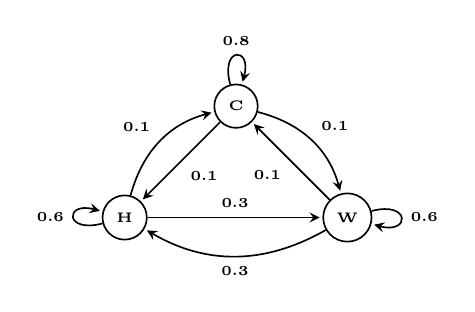
\begin{tikzpicture}[
				> = stealth, % arrow head style
				shorten > = 1pt, % don't touch arrow head to node
				auto,
				node distance = 2cm, % distance between nodes
				semithick, % line style
				font=\tiny\bfseries
				]
				
				\node[circle,draw] (qC) {C};
				\node[circle,draw] (qH) [below left of=qC] {H};
				\node[circle,draw] (qW) [below right of=qC] {W};
				
				\path[->] 	
				(qC) 	edge [loop above] node {0.8} ()
				edge [] node {0.1} (qH)
				edge [bend left] node {0.1} (qW)
				(qH) 	edge [loop left] node {0.6} ()
				edge [bend left] node {0.1} (qC)
				edge [] node {0.3} (qW)
				(qW)	edge [loop right] node {0.6} ()
				edge [bend left] node {0.3} (qH)
				edge [] node {0.1} (qC);
			\end{tikzpicture}
		\end{minipage}
		
		\begin{itemize}
			\item $\pi = [\pi_1, \pi_2, \ldots, \pi_n ]$ : la distribution initiale des probabilités des états
			\item $\sum_i \pi_i = 1$
			\item Ex. \expword{Calculer la probabilité $P(H\, W\, C\, C)$ lorsque $\pi = [0.1, 0.7, 0.2]$}
		\end{itemize}
	\end{frame}
	
	\begin{frame}
		\frametitle{ML pour TALN : \insertsection}
		\framesubtitle{\insertsubsection\ : Modèle de Markov caché}
		\begin{minipage}{.54\textwidth}
			\begin{itemize}
				%		\item Hypothèse de Markov
				%		\item $ P(q_i = a | q_1, \ldots, q_{i-1}) \approx P(q_i = a | q_{i-1}) $
				\item $Q = \{q_1, q_2, \ldots, q_n\}$ : états
				\item $A$ : matrice des probabilités de transitions où $\sum_j a_{ij} = 1,\, \forall i$
				\item $O = o_1 o_2 \ldots o_T$ : séquence des évènements observés (mots)
				\item $B = b_i(o_t)$ : probabilités d'observation (\keyword{probabilités d'émission}), chacune représente la probabilité de génération d'une observation $o_t$ dans un état $q_i$
			\end{itemize}
		\end{minipage}
		\begin{minipage}{.45\textwidth}
			%	\begin{figure}
				%		\hgraphpage{exp-hmm_.pdf}
				%		\caption{Exemple d'une représentation HMM \cite{2019-jurafsky-martin}}
				%	\end{figure}
			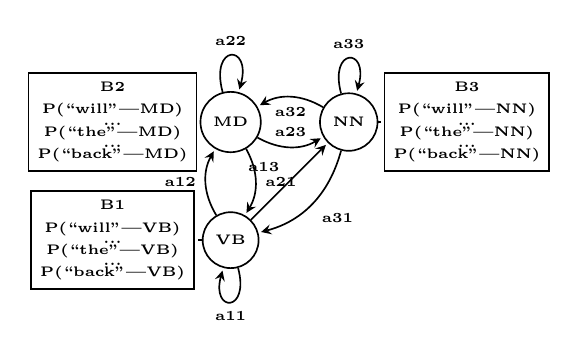
\begin{tikzpicture}[
				> = stealth, % arrow head style
				shorten > = 1pt, % don't touch arrow head to node
				auto,
				node distance = 1.5cm, % distance between nodes
				semithick, % line style
				font=\bfseries\fontsize{4}{4}\selectfont
				]
				
				\node[circle,draw] (q2) {MD};
				\node[align=center,draw] (q2e) [left of=q2] {B2\\ \\P(``will"|MD)\\...\\P(``the"|MD)\\...\\P(``back"|MD)};
				\node[circle,draw] (q3) [right of=q2] {NN};
				\node[align=center,draw] (q3e) [right of=q3] {B3\\ \\P(``will"|NN)\\...\\P(``the"|NN)\\...\\P(``back"|NN)};
				\node[circle,draw] (q1) [below of=q2] {VB};
				\node[align=center,draw] (q1e) [left of=q1] {B1\\ \\P(``will"|VB)\\...\\P(``the"|VB)\\...\\P(``back"|VB)};
				
				\path[->] 	
				(q1) 	edge [loop below] node {a11} ()
				edge [bend left] node {a12} (q2)
				edge [] node {a13} (q3)
				(q2) 	edge [loop above] node {a22} ()
				edge [bend left] node {a21} (q1)
				edge [bend right] node {a23} (q3)
				(q3)	edge [loop above] node {a33} ()
				edge [bend left] node {a31} (q1)
				edge [bend right] node {a32} (q2);
				
				\path[dashed] 	
				(q1) 	edge [] node {} (q1e)
				(q2) 	edge [] node {} (q2e)
				(q3) 	edge [] node {} (q3e);
				
			\end{tikzpicture}
		\end{minipage}
		
		\begin{itemize}
			\item $\pi = [\pi_1, \pi_2, \ldots, \pi_n ]$ : la distribution initiale des probabilités des états
			\item $\sum_i \pi_i = 1$
		\end{itemize}
		
	\end{frame}
	
	\begin{frame}
		\frametitle{ML pour TALN : \insertsection}
		\framesubtitle{\insertsubsection\ : Entraînement}
		
		\begin{itemize}
			\item Les états sont les tags (catégories) $t_i$
			\item Prenons \keyword{DEBUT} comme tag du début de la phrase
			\item Les observation $o_i$ sont les mots $w_i$
			\item \keyword{C} : Nombre des occurrences dans le corpus d'entraînement
		\end{itemize}
		
		\begin{block}{Entraînement du HMM pour étiquetage morpho-syntaxique}
			\[
			\text{Probabilité de transition : } P(t_i | t_{i-1}) = \frac{C(t_{i-1}, t_i)}{C(t_{i-1})} 
			\]\[
			\text{Probabilité d'émission : } P(w_i | t_i) = \frac{C(t_i, w_i)}{C(t_i)}
			\]\[
			\text{Distribution initiale : } \pi_i = P(t_i | DEBUT) = \frac{C(DEBUT, t_i)}{C(DEBUT)}
			\]
			
		\end{block}
	\end{frame}
	
	\begin{frame}
		\frametitle{ML pour TALN : \insertsection}
		\framesubtitle{\insertsubsection\ : Étiquetage (décodage des tags)}
		
		\begin{itemize}
			\item Étant donné 
			\begin{itemize}
				\item un modèle de Markov caché $\lambda = (A, B)$
				\item une séquence des observations (mots) : $w = w_1 w_2 \ldots w_n$
			\end{itemize}
			\item Estimer la séquence des étiquettes $\hat{t} = \hat{t}_1 \hat{t}_2 \ldots \hat{t}_n$
		\end{itemize}
		
		\begin{block}{Décodage des étiquètes en utilisant HMM}
			\[
			\hat{t} = \arg\max\limits_t P(t | w) = \arg\max\limits_t \frac{P(w|t) P(t)}{P(w)} = \arg\max\limits_t P(w|t) P(t)%\text{ tel que } t = t_1 t_2 \ldots t_n
			\]
			
			\[ 
			P(w | t) \approx \prod\limits_{i=1}^n P(w_i|t_i) 
			\hskip2cm
			P(t) \approx \prod\limits_{i=1}^n P(t_i|t_{i-1}) 
			\]
			
			\[
			\hat{t} = \arg\max\limits_t \prod\limits_{i=1}^n P(w_i|t_i) P(t_i|t_{i-1})
			\]
		\end{block}
	\end{frame}
	
	\begin{frame}
		\frametitle{ML pour TALN : \insertsection}
		\framesubtitle{\insertsubsection\ : Viterbi}
		\vspace{-6pt}
		\begin{block}{Viterbi }
			\scriptsize
			\begin{algorithm}[H]
				\KwData{$w = w_1 \ldots w_T$, HMM $\lambda = (A, B)$ avec $N$ états}
				\KwResult{$meilleur\_chemin$, $prob\_chemin$}
				
				Créer une matrice $viterbi[N, T]$\;
				
				\Pour{état $ s = 1 \ldots N$}{
					$viterbi[s, 1] = \pi_s * b_s(w_1);\, backpointer[s, 1] = 0$ \;
				}
				
				\Pour{$ t = 2 \ldots T$}{
					\Pour{état $ s = 1 \ldots N$}{
						$viterbi[s, t] = \max\limits_{s'=1}^N viterbi[s', t-1] * a_{s',s} * b_s(w_t)$\;
						$backpointer[s, t] = \arg\max\limits_{s'=1}^N viterbi[s', t-1] * a_{s',s} * b_s(w_t)$\;
					}
				}
				
				$prob\_chemin = \max\limits_{s=1}^N viterbi[s, T];\, pointeur\_chemin = \arg\max\limits_{s=1}^N viterbi[s, T]$\;
				
				$meilleur\_chemin$ est le chemin qui commence par $pointeur\_chemin$ et qui suit $backpointer$
				
				\Return $meilleur\_chemin$, $prob\_chemin$\;
				
			\end{algorithm}
		\end{block}
		
	\end{frame}
	
	\subsection{MEMM}
	
	\begin{frame}
		\frametitle{ML pour TALN : \insertsection}
		\framesubtitle{\insertsubsection}
		
		\begin{itemize}
			\item On note $x_{n}^{m} = x_n x_{n+1} \ldots x_{m-1} x_m$
			\item Étant donné 
			\begin{itemize}
				\item une séquence des observations (mots) : $w = w_1 w_2 \ldots w_n$
				\item un ensemble des caractéristiques $f$ sur les séquences (comme : mot en majuscule)
			\end{itemize}
			\item Estimer la séquence des étiquettes $\hat{t} = \hat{t}_1 \hat{t}_2 \ldots \hat{t}_n$
		\end{itemize}
		
		\begin{block}{Décodage des étiquettes en utilisant MEMM}
			\[
			\hat{t} = \arg\max\limits_t P(t | w) = \arg\max\limits_t \prod\limits_{i}  P(t_i | w_i, t_{i-1})
			\]
			
			\[
			\hat{t} = \arg\max\limits_t \prod\limits_{i}  
			\frac{exp\left(\sum_j \theta_j f_j(t_i, w_{i-l}^{i+l}, t_{i-k}^{i-1})\right)}%
			{\sum_{t' \in tags} exp\left(\sum_j \theta_j f_j(t'_i, w_{i-l}^{i+l}, t_{i-k}^{i-1})\right)}
			\]
			
		\end{block}
		
	\end{frame}
	
	\subsection{RNN}
	
	\begin{frame}
		\frametitle{ML pour TALN : \insertsection}
		\framesubtitle{\insertsubsection\ : Exemples}
		
		\vgraphpage{seq_class_RNN_exp.pdf}
		
	\end{frame}
	%===================================================================================
	\section{Attention}
	%===================================================================================
	
	\begin{frame}
		\frametitle{ML pour TALN}
		\framesubtitle{\insertsection}
		
		\begin{itemize}
			\item Le mécanisme d'attention sert à donner plus d'importance à une partie des données d'entrée plus que d'autres.
			\item Il améliore la capture de l'information à long terme
		\end{itemize}
		
	\end{frame}
	
	\subsection{Seq2Seq}
	
	\begin{frame}
		\frametitle{ML pour TALN : \insertsection}
		\framesubtitle{\insertsubsection}
		
		\hgraphpage{seq2seq_exp.pdf}
	\end{frame}
	
	\subsection{Seq2Seq avec attention}
	
	\begin{frame}
		\frametitle{ML pour TALN : \insertsection}
		\framesubtitle{\insertsubsection}
		
		\hgraphpage{seq2seq_attention.pdf}
		
	\end{frame}
	
	\subsection{Types d'attention}
	
	\begin{frame}
		\frametitle{ML pour TALN : \insertsection}
		\framesubtitle{\insertsubsection}
		
			\[Q \in \mathbb{R}^{n \times d}, \, K \in \mathbb{R}^{m \times d}, \, a(Q, K) \in \mathbb{R}^{n \times m}, V \in \mathbb{R}^{m \times v} \]
		
		\begin{itemize}
	
		\item Dot product (\textbf{tf.keras.layers.Attention})
		
		$ a(Q, K) = Q \cdot K^\top $
		
		\item Scaled dot product 
		
		$a(Q, K) = \frac{Q \cdot K^\top}{\sqrt{d}}$
		
		\item Cosine similarity
		
		$ a(Q, K) = \frac{Q \cdot K^\top}{||Q|| \, ||K||} $
		
		\item Additive attention (\textbf{tf.keras.layers.AdditiveAttention})
		
		Bahdanau Attention
		
		$ a(Q, K) = W_v^\top \cdot \tanh(W_q Q + W_k K) $
	\end{itemize}
		
	\end{frame}
	
	
	\subsection{Transformers}
	
	\begin{frame}
		\frametitle{ML pour TALN : \insertsection}
		\framesubtitle{\insertsubsection\ : Attention multi-têtes (Multi-Head Attention)}
		\vspace{-0.5cm}
		\begin{figure}
			\centering
			\hgraphpage[0.9\textwidth]{multi_head_att_.pdf}
			\caption{Attention multi-têtes \cite{2017-vaswani-al}}
		\end{figure}
	\end{frame}

	\begin{frame}
		\frametitle{ML pour TALN : \insertsection}
		\framesubtitle{\insertsubsection\ : Attention multi-têtes (Multi-Head Attention)}
		\begin{itemize}
			\item Q, K et V sont appris avec un MLP
		\end{itemize}
		\[Q \in \mathbb{R}^{n \times d}, \, K \in \mathbb{R}^{m \times d}, \, MultiHead \in \mathbb{R}^{n \times d_{model}}, V \in \mathbb{R}^{m \times v} \]
		
		\[W^Q_i \in \mathbb{R}^{d_{model} \times d}, \,  W^K_i \in \mathbb{R}^{d_{model} \times d}, \, W^V_i \in \mathbb{R}^{d_{model} \times v}, \, W^O \in \mathbb{R}^{hv \times d_{model}}\]
		
		
		\[MultiHead(Q, K, V) = Concat(head_1, \ldots, head_h) \cdot W^O\]
		
		\[head_i = Attention(Q W^Q_i, K W^Q_i, V W^V_i)\]
	\end{frame}


	\begin{frame}
		\frametitle{ML pour TALN : \insertsection}
		\framesubtitle{\insertsubsection\ : Attention multi-têtes (Multi-Head Attention)}
		\vspace{-0.4cm}
		\begin{figure}
			\centering
			\hgraphpage[0.35\textwidth]{transformers_.pdf}
			\caption{Architecture des transformers \cite{2017-vaswani-al}}
		\end{figure}
	\end{frame}

	
	\insertbibliography{TALN03}{*}
	
\end{document}

